% TODO Use 'features' instead of 'information'.

\documentclass[abstract=true,caption=above]{scrreprt}
\usepackage[utf8]{inputenc}
\usepackage[american]{babel}

\usepackage[backend=biber,style=numeric]{biblatex}
\addbibresource{references.bib}

\usepackage{graphicx}
\graphicspath{ {images/} }
\usepackage{subcaption}
\setcapindent{0em}
\usepackage{wrapfig}

% \usepackage{endfloat}

\usepackage{amsmath}

% For tables exported from pandas.
\usepackage{booktabs}

% For typesetting urls.
\usepackage[hidelinks]{hyperref}

% Title Page
\subject{Bachelor's Thesis}
\title{Predicting Spread Prices on VIX Futures with Deep Learning}
\author{Thomas Leyh}
\date{September 8th, 2017}
\publishers{
\includegraphics[width=0.5\linewidth]{Uni_Logo-Grundversion_E1_A4_CMYK.pdf}\\
			\vspace{1cm}
			University of Freiburg \\
			Department of Computer Science \\
			Computer Vision Group \\
			Prof. Dr. Thomas Brox}
		
\dedication{%
	Many thanks to Konstantin Andreyev and Javdat Umarov from Beneficious Investment Management for introducing me to the world of finance and for all the advice they have given me.
}

\begin{document}
	
\maketitle

\pagenumbering{gobble}

\chapter*{Abstract}

The CBOE's Volatility Index (VIX) is a popular measure of financial volatility. Since 2004 it is possible to trade futures directly on the index. This work explores ways to make predictions on these futures' prices with deep learning, a machine learning technique that became increasingly popular during the last few years. Focus of this work is the prediction of butterfly spread prices using only few inputs derived from the futures itself. Several approaches failed, leading to the conclusion that deep learning -- at least under these constraints -- will not yield satisfying results.

\vspace{1in}

\section*{Deutsche Übersetzung}

Der CBOE's Volatility Index (VIX) stellt eine Messgröße zur Schwankungsanfälligkeit des S\&P~500 dar. Seit 2004 können auf diesem Index aufbauende Futures gehandelt werden. Thema dieser Arbeit ist die Vorhersage der entsprechenden Preise unter Verwendung von Deep Learning, einer seit Kurzem sehr populären Technik aus dem Repertoire des maschinellen Lernens. Insbesondere stehen sogenannte Butterfly Spreads im Fokus, deren zukünftige Preise allein aus den Futures selbst geschätzt werden sollen. Die unter diesen Bedingungen unternommenen Versuche schlugen fehl. Entsprechend ist zu erwarten, dass Deep Learning -- zumindest unter ähnlichen Bedingungen -- in diesem Bereich wenig erfolgversprechend ist.

\chapter*{Declaration}

I hereby declare, that I am the sole author and composer of my Thesis and that no other sources or learning aids, other than those listed, have been used. Furthermore, I declare that I have acknowledged the work of others by providing detailed references of said work.

I hereby also declare, that my Thesis has not been prepared for another examination
or assignment, either wholly or excerpts thereof.

\parbox{\textwidth}{
	\vspace{2cm}
	\parbox{7cm}{
		\rule{4cm}{1pt}\\
		Place, date
	}
	\hfill
	\parbox{7cm}{
		\rule{6cm}{1pt}\\
		Signature
	}
}

\tableofcontents

\pagenumbering{roman}
\setcounter{page}{1}

\listoffigures
\listoftables

\chapter{Introduction}
\pagenumbering{arabic}
\setcounter{page}{1}
Working on financial problems is interesting on many levels. There is a large number of markets and it is easy to get the corresponding data even from years back.\footnote{%
	Although there are differences in the quality of the data resulting in a gap between freely available and commercial sources.}
What is measured is mostly \emph{value} and even though this is only an abstract concept its quantified by currencies which again opens the possibility of comparison between markets, assets etc.
There is also a large number of mathematical models and techniques often with intriguing results.

But even though all this formalization conveys a sense of order, one must not forget that markets are something created by humans. Therefore financial research is also related to the social sciences and besides all assumed efficiencies is subject to human emotion. As a result financial markets are ever-changing and nonlinear in their behavior.

Machine learning is about algorithms to enable computers to learn from existing data, allowing them e.g. to make predictions. In theory this could partly relieve human experts from adapting to market changes. For modeling financial data especially one technique might be useful: artificial neural networks with multiple layers -- recently rebranded as \emph{deep learning} -- already showed promising results in other works (e.g. \cite{Niaki-2013}).

First some necessary background for finance as well as deep learning is given. Using this knowledge, a description of the problem itself follows. Next comes the experimental part, evaluating data structure and model selection. Finally the results and findings are summarized, concluding this work.

On a technical note, the underlying code was written in Python~3 using Google's TensorFlow machine learning library.\cite{tensorflow2015-whitepaper} \\
The code is available at: \url{https://github.com/leyhline/vix-term-structure}

\section{Financial background}
\label{sec:financial-background}

The financial sector is large and there is lots of theory involved. The most important terms for understanding this work are introduced below.

\paragraph{Volatility} -- in a financial context -- is the annualized standard deviation of returns. Actual volatility is hard to measure because one does not know beforehand about the returns of a financial instrument. Instead one can calculate \emph{implied volatility} as a more subjective measure using the current market price on some pricing model.\footnote{%
	The subjectivity stems from the selected model. Often the Black-Scholes model is used.}\cite{wilmottwiki-volatility} 

\paragraph{The CBOE Volatility Index} got first introduced in 1993 by the Chicago Board Options Exchange. Its ticker symbol is ``VIX'' which will be used instead of the full name during this work. As the name suggests it is a measure of volatility (\emph{implied volatility} to be more precise). Since 2003 it is based on the S\&P 500, an important index of the American stock market. For calculation details see the VIX Whitepaper \cite{VIX}. The VIX is largely used in financial research as well as in practice and got labeled ``fear index'' because a high value can be interpreted as a high risk of sharp market movements. Since March 2004 it is possible to trade futures contracts on the VIX which allows investing in these volatilities.

\begin{figure}
	\centering
	\includegraphics[width=0.8\linewidth]{vix}
	\caption[VIX from year 2006 to 2016]{Adjusted closing value of the VIX from year 2006 to 2016. Note the large spike at the end of 2008 when the global financial crisis was in full swing.}
	\label{fig:vix}
\end{figure}


\paragraph{Futures contracts} are a standard exchange-traded contract which guarantee the delivery of some underlying\footnote{%
	Because there is some underlying asset, futures belong to the family of derivative products.} 
commodity, interest rate or equity at some specified future date (expiry).\cite{wilmottwiki-futures}
They often just get called ``futures''. Because of their standardization and the resulting ease of trading, large markets formed around them. Specifically VIX futures allow for trading volatility expectations of some future date. More information about the structure of VIX futures will be presented in section~\ref{sec:aao-input-data}. One can invest in futures by placing \emph{long} or \emph{short positions}. 

By holding a long position its holder is obliged to buy the underlying assert at expiry and will hence profit from price increases. In contrast, short positions are more abstract. Their immediate meaning comes from the obligation to deliver the underlying asset at expiry. But even with no such assets at hand one can hold short positions and profit from declining prices because of the margin when purchasing its asset later. They often get abbreviated simply as ``long'' and ``short''. Intuitively it is like betting, where one can bet on rising (long) or falling (short) prices. But making such simple bets contains much risk and there are further strategies for placing these positions in a safer way.

\paragraph{Butterfly spreads} are such a strategy which will be used during this work. The general idea is simple: By mixing long and short positions on different conditions the risk of loss -- but also the profit -- gets limited. The specific usage of butterfly spreads on VIX futures gets explained in section~\ref{sec:problem-description}.

\section{Deep Learning}
\label{sec:deep-learning}

Even though the term ``deep learning'' is quite young the general architecture of its models existed for many decades. One of the first implementations might be the \emph{perceptron} by Rosenblatt in 1958. Because of its inspiration by the human brain and its connections to neuroscience the name \emph{artificial neural networks} (ANN) is most prevalent for this model family.

An especially interesting characteristic is stated in the \emph{universal approximation theorem}.\cite{Hornik-1989} It says that given enough hidden units such a network can approximate any function from one finite-dimensional space to another. But despite this theoretical representational power it is not guaranteed that one can successfully train such a network to learn the desired mapping. Because of this ANNs largely got ignored until some advantages in theory, computational power as well as larger databases allowed for breakthroughs in fields like computer vision, speech synthesis and natural language processing. With these, new interest in this model family was kindled.\cite[p.\,12ff.]{Goodfellow-et-al-2016}

\begin{figure}
	\centering
	\includegraphics[width=0.7\linewidth]{images/MultiLayerNeuralNetworkBigger_english}
	\caption[Diagram of a multi-layer feedforward artificial neural network]{%
		Diagram of a simple feedforward artificial neural network with three input nodes, one hidden layer (also with three nodes) and two output nodes. Each arrow represents a trainable weight.{\cite{wikimedia-fnn}}
	}
	\label{fig:multilayerneuralnetwork}
\end{figure}

In this work a simple architecture called \emph{feedforward neural network} (FNN), as depicted in figure~\ref{fig:multilayerneuralnetwork}, is used. In such models information only flows forward. There can be multiple hidden layers with associated weights which introduce nonlinearities. These weights are trained interatively by a technique called backpropagation where some loss function at the output of the network gets minimized by propagating the loss backwards to its beginning. The number of hidden layers is often called the \emph{depth} of a network while the maximum number of units of one such layer is called \emph{width}.

\section{Problem description}
\label{sec:problem-description}

With this, the precise definition of this thesis' goal is:

\begin{quote}
	Using the term structure and possibly additional information of a certain date to predict the corresponding spread prices of some later term.
\end{quote}

The benefit of this prediction becomes evident when looking at figure~\ref{fig:term-structure}. Most term structures have a nearly concave or convex shape. Deviations (like some small dents in the curve) are a sign of market inefficiencies that might get corrected. By investing at the right time one can gain profits if this correction takes place. A prediction might help estimating time and position of meaningful investments as well as holding time.

\begin{figure}
	\centering
	\begin{subfigure}{0.45\linewidth}
		\includegraphics[width=\linewidth]{term-structure}
		\caption{}
		\label{fig:term-structure-yearly}
	\end{subfigure}
	\begin{subfigure}{0.45\linewidth}
		\includegraphics[width=\linewidth]{term-structure-crisis}
		\caption{}
		\label{fig:term-structure-crisis}
	\end{subfigure}\\
	\caption[Exemplary term structures of VIX futures]{%
		Exemplary term structures of VIX futures. Each line represents eight futures' prices with their month of expiration given on the x-axis. The y-axis represents their respective price. Note how in (a) each term structure is (nearly) concave. Most of the data has a similar structure. However, in time of crisis this might be different: (b) shows the term structures during November 2008, at the height of the global financial crisis. The red lines represent futures that are closer to their expiration. Their shape if often similar to convex functions. This is a form of \emph{mean reversion}{\footnotemark} where the volatility is expected to converge to some average value in the future.}
	\label{fig:term-structure}
\end{figure}
\footnotetext{A very popular and useful concept in finance as well as in daily life.}

These investments itself take place in form of butterfly spreads (intuitively described in section~\ref{sec:financial-background}). One has to distinguish between \emph{long spreads} (opening two long positions and respectively one short position at its neighboring futures) and the contrasting \emph{short spreads} (opening two short positions and respectively one long position at its neighboring futures). If there are $M$ futures' prices for a certain date and $m_i$ is the price of the $i$-th one, this results in the following definition:

\begin{subequations}
	\begin{align}
		\label{eq:long-spread}
		v^{long}_i &= 2m_i - m_{i-1} - m_{i+1} & \text{(long spread price)}
		\\
		\label{eq:short-spread}
		v^{short}_i &= -2m_i + m_{i-1} + m_{i+1} & \text{(short spread price)}
	\end{align}
\end{subequations}

One can easily see that:
\begin{equation}
	\label{eq:spread-correlation}
	v^{long}_i = -v^{short}_i 
\end{equation}
 
Moreover, there only exists a spread price for $i \in \{2,\dots,M-1\}$. In our data, most of the time a term structure of futures consists of eight prices. Therefore we have $M=8$ and six corresponding spread prices (spanning their own term structure). See figure~\ref{fig:longspread} for an example with long spreads.

\begin{figure}
	\centering
	\includegraphics[width=0.8\linewidth]{images/long_spread}
	\caption[Term structure and corresponding spread prices from Feb 29, 2012]{%
		Term structure (green) and its corresponding long spread prices (blue) also forming their own term structure for February 29th, 2012.}
	\label{fig:longspread}
\end{figure}

But why use these butterfly spreads instead of investing in the futures directly? Recalling the goal of this work, it is about exploiting the term structure. Therefore the absolute value of the futures' prices is not of primary interest but the derived curvature. Butterfly spreads are a well-tried method allowing such an approach.

\newpage

When using machine learning, one has to do the following tasks: \cite{automl-2017}

\begin{enumerate}
	\item Preprocess the data
	\item Select appropriate features
	\item Select an appropriate model family
	\item Optimize model hyperparameters
	\item Postprocess machine learning models
	\item Critically analyze the results obtained
\end{enumerate}

While the title of this work already implies a model family from the subfield of deep learning -- specifically feedforward neural networks (FNNs) as mentioned in section~\ref{sec:deep-learning} -- the remaining points are determined in the course of the next chapters.

Of particular importance is the structure of the data (1. and 2.) because the remaining tasks have to be adjusted accordingly. There are two output representations this work will explore in detail: Predicting all spread prices at once (chapter~\ref{ch:all-at-once}) and predicting only a single spread price (chapter~\ref{ch:one-at-once}). The specific network structure and the corresponding hyperparameters are investigated in the respective chapters.

\chapter[First approach: Predicting all spread prices at once]{First approach: \\  Predicting all spread prices at once}
\label{ch:all-at-once}
The general idea behind this approach is simple: There exists one network which takes the futures' term structure as input and outputs a prediction of spread prices. If not specified otherwise the prices of the next business day are predicted. This is quite similar to figure~\ref{fig:longspread} where the green data points are the input and the blue data points -- but now for the next day! -- the output. Ideally one just has to find optimal hyperparameters.

The first part of this section will be about getting familiar with the data itself. This includes a general description as well as the handling of problematic data points.
Thereafter the network architecture as well as the tunable hyperparameters will be introduced more formally.
At last the the results of this approach are presented in a detailed manner.

\section{Data description and data handling}
\label{sec:aao-data-handling}

Primarily, the available data are the prices of VIX futures since they were first issued in 2004. Supplementary there is data about the VIX itself as well as additional information about the futures: their symbol and their precise date of expiration. All of these are sampled on a daily interval. There is also minutely data available which will not be used unless explicitly mentioned.

\subsection{Input data (term structure)}
\label{sec:aao-input-data}

The set of term structure data includes 3,304 samples in total from March 26th, 2004 to May 5th, 2017. Each term structure consists of three up to eight legs. The legs symbolize the months when the respective future expires. The specific date of expiration is always a workday in the middle of this month. For an example term structure see table~\ref{tab:single-termstructure} and for a graphical overview over the whole data set see figure~\ref{fig:termstructures}. Notice how similar the legs look to each other and to the VIX from figure~\ref{fig:vix}. To make the curvature between the term structures' legs more explicit their difference is calculated and used as network input.

\begin{table}
	\centering
	\caption[Single term structure with expiration dates (February 29th, 2012)]{A single term structure with expiration dates (February 29th, 2012) and corresponding long prices. The eight values are the futures' current prices for the next eight months. The expiration row shows the date the respective future expires. After expiration one can not invest in this future anymore.}
	\begin{tabular}{lllllllll}
	\toprule
	{} &      M1 &      M2 &      M3 &      M4 &      M5 &      M6 &      M7 &      M8 \\
	\midrule
	Value      &   21.00 &   23.99 &   25.60 &   26.50 &   27.75 &   28.40 &   29.05 &   29.25 \\
	Expiration &  Mar 21 &  Apr 18 &  May 16 &  Jun 20 &  Jul 18 &  Aug 22 &  Sep 19 &  Oct 17 \\
    \midrule	
    Long Price &         &    1.38 &    0.71 &   -0.35 &    0.60 &    0.00 &    0.45 &         \\
	\bottomrule
	\end{tabular}
 	\label{tab:single-termstructure}
\end{table}

\begin{figure}
	\centering
	\includegraphics[width=0.9\linewidth]{termstructures}
	\caption[Complete data set of term structures]{%
		Complete data set of term structures. Each term structure consists of at most eight legs (M1 to M8) where M1 is closest to expiration (blue). For most of the data -- except in times of crisis -- the legs with later expiration (green) have a higher price. Furthermore the general shape of the data is very similar between legs as well as similar to the VIX itself (see figure~\ref{fig:vix}).}
	\label{fig:termstructures}
\end{figure}

One problem for this task is missing data. If there are values for all eight months of a term structure like in table~\ref{tab:single-termstructure} this is a \emph{complete} sample. Consequently, when there are values missing it is an \emph{incomplete} sample. As seen in figure~\ref{fig:some-nice-graphics} there are especially many incomplete samples in earlier years. Because trading of futures just started it was not as established as of now. Futures are issued per month. But even though this happens regulary for each consecutive month since 2012 this was not always the case before. However, this regularity is necessary for a complete term structure. Removing all incomplete samples would shrink the dataset by $35\%$. 
By removing all samples before October 23th, 2006 only samples with up to two missing legs are left. This shrinks the data set by just $20\%$ resulting in 2,656 remaining samples. The remaining incomplete samples need to be handled by the network itself.

\begin{figure}
		\centering
	\begin{subfigure}{0.45\linewidth}
		\includegraphics[width=\linewidth]{number_of_samples}
		\caption{Number of samples by year}
		\label{fig:missing-values}
	\end{subfigure}
	\begin{subfigure}{0.45\linewidth}
		\includegraphics[width=0.95\linewidth]{missing_values}
		\caption{Distribution of missing values}
		\label{fig:weekdays}
	\end{subfigure}
	\caption[Number of samples by year and distribution of missing values]{%
		While a whole term structure consists of eight legs there is often less data available, especially in earlier years. Even though there are less samples from 2004 to 2006 there is a larger number of \emph{incomplete} term structures, often missing up to five legs.}
	\label{fig:some-nice-graphics}
\end{figure}

\subsection{Target data (long spread prices)}
\label{sec:aao-target-data}

For training a network one needs inputs as well as corresponding targets. While the term structure data set holds the necessary inputs, it is easy to calculate the target by applying \eqref{eq:long-spread} thus getting the long spread prices (see table~\ref{tab:single-termstructure}).\footnote{%
	Because of \eqref{eq:spread-correlation} it is sufficient to either calculate long spreads \emph{or} short spreads.}
For a complete term structure we get a complete set of spread prices consisting of six values.
Obviously the targets are the spread prices of the next term. Otherwise the network will not learn to make a prediction but an approximation of the applied formula. Because the term structure is the calculatory basis of the spread prices, they suffer from the same problem of missing data. Furthermore one has to exercise caution when expiration is close, so prediction is not made for already expired values.

\subsection{Seasonality}
\label{sec:seasonality}

As the original problem is finding inefficiencies in the term structure the network needs to be able to predict some recurring patterns. Therefore one might need some additional prior introducing seasonality. Some options are:

\newpage

\begin{itemize}
	\item The day of the month (1st to 31st)
	\item The month itself (Jan to Dec)
	\item The days until expiration of the term structure's first leg (0 to 34; see figure~\ref{fig:daystoexpiration})
\end{itemize}

The latter one -- the days until expiration -- has a nice property that is hopefully\footnote{%
Understanding what exactly a network actually learns is very difficult. One can not simply assume the same behavior as for humans. Most of the time one can only \emph{hope} the own choices were correct.}
advantageous in this context: 
There exist a total order. The former two are categorical by nature, e.g. without knowing about the year, January is \emph{not smaller} than February. But it is certainly possible to count down the days until expiration. Therefore it is appropriate to model these as a simple natural number at the network's input. For the alternatives is might have been necessary to use more verbose representations like a one-hot vector.\footnote{%
	A \emph{one-hot vector} is a binary vector with the same length as there are classes. All entries are $0$, except one which holds the value $1$. The position of this $1$ denotes the corresponding class.}

\begin{figure}
	\centering
	\includegraphics[width=0.9\linewidth]{days_to_expiration}
	\caption[Distribution of days to expiration for the termstructures' first leg]{%
		Distribution of days to expiration for the term structures' first leg.}
	\label{fig:daystoexpiration}
\end{figure}

\begin{table}
	\centering
	\caption[Descriptive statistics for futures and spread prices]{Common descriptive statistics for futures, their legs' difference and spread prices.}
	\begin{tabular}{lrrrrrrr}
		\toprule
		{} &  Mean &  Std. &    Min. &   25\% &   50\% &   75\% &  Max. \\
		\midrule
		Futures & 22.38 & 6.91 &  10.24 & 17.55 & 20.70 & 25.70 & 67.90 \\
		Difference & 0.38 & 1.00 & 21.10 & 0.07 & 0.40 & 0.75 & 5.45 \\
		Spread prices  &  0.11 & 0.74 & -13.68 & -0.10 &  0.13 &  0.36 &  4.90 \\
		\bottomrule
	\end{tabular}
	\label{tab:descriptive-stats}
\end{table}

\subsection{Normalization}

Looking at the most common descriptive statistics for input and target data in table~\ref{tab:descriptive-stats} -- especially the quantiles -- the spread prices are usually smaller than the futures by two orders of magnitude. And even for the differences of the futures' legs there are some outliers. This will not necessarily pose a problem but nevertheless \emph{optional} normalization is introduced by:

\begin{equation}
	X' = \frac{X - \bar{X}}{X_{max} - X_{min}} \quad \text{where $\bar{X}$ is the mean.}
\end{equation}

Hence, the resulting values of $X'$ will be in range $[0,1]$.

When explicitly mentioned am alternative formula for normalization is used, leading to zero mean and unit variance:

\begin{equation}
	\label{eq:normalization2}
	X'' = \frac{X - \bar{X}}{Std(X)} = \frac{X - \bar{X}}{\sqrt{Var(X)}}
\end{equation}

\subsection{Validation and test set}
\label{sec:aao-validation-and-test-set}

For validating the performance of deep networks the most widespread approach is to use one part of the data for tuning the hyperparameters introduced in section~\ref{sec:hyperparameters} (the \emph{validation set}) and one part for evaluating the final model (the \emph{test set}). In this work $15\%$ of the data will be used for validation and test set each. 

Looking at figure~\ref{fig:termstructures} it becomes evident that there is a temporal connection between areas of low and high price: If you look at some sample with low priced futures there is a high probability that samples next to this one also have a low price and vice versa. Therefore choosing completely random samples for validation and testing will result in datasets highly similar to the training set. But choosing one large connected chunk will result in hyperparameters fitted only to this timeframe. Choosing a tradeoff, test and validation set will be chosen by taking two chunks of data from different locations of the original data each, as shown in figure~\ref{fig:validation-and-test-set}.

\begin{figure}
	\centering
	\includegraphics[width=0.9\linewidth]{images/validation-and-test-set}
	\caption[Splitting whole dataset into training, validation and test set]{Splitting the whole dataset into training, validation and test set. The top figure shows the futures' prices for the next eight months (M1 to M8) of expiration forming the term structure. The bottom figure shows the corresponding spread prices. While the green area shows the data used for validation the red area is used for testing. The remaining data is used for training.}
	\label{fig:validation-and-test-set}
\end{figure}


\section{Network architecture}
\label{sec:aao-network-architecture}

A feedforward neural network is one oft the simplest architectures used in deep learning. First, there will be some definitions describing the network as well as some intuitions about training of neural networks. Thereafter the hyperparameters for tailoring the network to the problem are introduced. To prevent clueless searching over all of these some defaults are adopted. Finally, as already mentioned, the network needs to handle missing data. Some simple approach introducing an additional layer at the networks' output is introduced.

\subsection{Definitions}

The feedforward neural network can formally be described as a sequence of matrix-vector multiplications. Let $L$ be the number of hidden layers where $l \in \{1,\dots,L\}$ is the hidden layer's index. For a layer $l$ there is an input vector $\mathbf{z}^{(l)}$, an output vector $\mathbf{y}^{(l)}$ as well as a weight matrix $W^{(l)}$ and a bias vector $\mathbf{b}^{(l)}$. The input layer be $\mathbf{x} = \mathbf{y}^{(0)}$ and the output $\mathbf{t} = \mathbf{y}^{(L+1)}$. Furthermore there is an activation function $f^{(l)}$. At the output $f^{(L+1)}$ is typically the identity function.

Inference is done by the following operations for $l \in \{1,\dots,L+1\}$:

\begin{align}
	\label{eq:layer-input}
	\mathbf{z}^{(l)} &= W^{(l)\top} \mathbf{y}^{(l-1)} + \mathbf{b}^{(l)} \\
	\label{eq:layer-output}
	\mathbf{y}^{(l)} &= f^{(l)}(\mathbf{z}^{(l)})
\end{align}

Each hidden layer can have an arbitrary width greater zero. A layer's width is the length of the vector $\mathbf{y}^{(l)}$. In this work each hidden layer has the same width. Let this be the network's width $K$. Accordingly, the number of hidden layers $L$ is the network's depth.

For training -- this corresponds to optimizing $W$ and $\mathbf{b}$ -- the \emph{back-propagation} algorithm along with an optimization method like \emph{stochastic gradient descent} is used. Therefore a scalar loss function $J(\mathbf{t}, \mathbf{\hat{t}})$ is introduced, comparing the output of the network $\mathbf{t}$ to the target $\mathbf{\hat{t}}$. By iteratively computing the gradient with respect to the parameters $W$ and $\mathbf{b}$ for $J$ as well as for the activation functions $f^{(l)}$ backwards through the network one can optimize each layer's parameters. For further details see \cite{Rumelhart-1986a} and \cite[p.\,204ff.]{Goodfellow-et-al-2016}.

\subsection{Hyperparameters}
\label{sec:hyperparameters}

These definitions result in a number of tunable hyperparameters, potentially affecting the network's performance:
\begin{itemize}
	\item Activation functions $f^{(l)}$
	\item Loss function $J$
	\item Optimization method (and corresponding hyperparameters)
	\item Weight initializations (choosing initial values for $W^{(l)}$)
	\item Network depth $L$
	\item Network width $K$
\end{itemize}

While for some of these it is relatively easy to find some good values or there is some reasonable default, others are highly dependent on the problem and the data. For these, one has to extensively search for optimal values while constantly validating the performance. 

\paragraph{Activation functions.}
(also called hidden units when used together with their input from \eqref{eq:layer-input}) \\
One can read in \cite[p.\,191]{Goodfellow-et-al-2016}:
\begin{quote}
	``The design of hidden units is an extremely active area of research and does not yet have many definitive guiding theoretical principles.''
\end{quote}

\begin{wrapfigure}[8]{r}{0.3\textwidth}
	\vspace{-1em}
	\fbox{%
		\begin{minipage}{0.3\textwidth}\centering
			\includegraphics[width=\textwidth]{images/rectifier}
			\vspace{-20pt}
			\caption[Rectifier function]{%
				Rectifier \\ function $f(z)=\max(0,z)$}
			\label{fig:rectifier}
	\end{minipage}}
\end{wrapfigure}

Although directly followed by:
\begin{quote}
	``Rectified linear units are an excellent default choice of hidden unit.''
\end{quote}

A \emph{rectified linear unit} (ReLU) uses the activation function $f(z)=\max(0,z)$ (also called \emph{rectifier}, see figure~\ref{fig:rectifier}) meaning for $z \leq 0$ it always outputs zero. This offers some nice and simple properties especially regarding its derivative.\footnote{%
	The derivative is 0 across half its domain and 1 in the other. Furthermore the second derivative is 0 almost everywhere eliminating second-order effects.}
Using this function should ensure reasonable performance.

An alternative might be using \emph{scaled exponential linear units} (SELUs) as activations thus building a \emph{self-normalizing neural network}.\cite{DBLP:journals/corr/KlambauerUMH17} This is a very recent approach aiming for mapping the mean and variance from each layer to the next one. They explicitly try to solve some shortcoming of feedforward neural networks, often showing effective regularization properties. The SELU activation function is given by:

\begin{equation}
	\label{eq:selu}
	f(z) = \lambda
	\begin{cases}
	z & \text{if } z > 0 \\
	\alpha e^z - \alpha & \text{if } z \leq 0
	\end{cases}
\end{equation}

The corresponding paper suggests using $\alpha = 1.6733$ and $\lambda = 1.0507$ implying zero mean and unit variance. These are most effective if the training data has zero mean and unit variance, too, which can be accomplished by normalization using equation~\eqref{eq:normalization2}.

\paragraph{Loss function.}
This can be chosen quite conservatively, too. To penalize larger derivations from the target value proportionally more the \emph{mean squared error} (MSE) is used:
\begin{equation}
	\label{eq:mse}
	J(\mathbf{t}, \mathbf{\hat{t}}) =
	\frac{1}{n} \sum_{i=1}^{n}(t_i - \hat{t}_i)^2 \quad
	\text{where } n \text{ is the length of vector } \mathbf{t}.
\end{equation}

\paragraph{Optimization method.}
Most of the time \emph{stochastic gradient descent} (SGD) or some extension is chosen. The general idea is to use the gradient $\nabla_{\theta}J(\theta)$ of a function $J$ with parameters $\theta$ to find the direction (in parameter space) with the steepest descent. By updating the parameters iteratively with small steps\footnote{%
	Typically some value $\tau < 1$ is chosen like $0.01$ or $0.001$.}
of size $\alpha$ one is guaranteed to find a local minimum:

\begin{equation}
	\theta^{(i+1)} = \theta^{(i)} - \alpha \nabla_{\theta}J(\theta^{(i)})
\end{equation}

This formula describes the general gradient descent algorithm. As for the stochastic part, one takes a specific number of samples from the dataset -- called the \emph{batch size} -- and updates the parameters after evaluating just this sample. In deep learning SGD is applied with respect to weights $W$ and bias $\mathbf{b}$ for loss and activation functions. Because of the non-convex structure of neural networks finding a local minimum (instead of a global one) is acceptable. In practice this works reasonably well.

In this work primary the \emph{Adam}\footnote{``\dots the name Adam is derived from adaptive moment estimation.''} algorithm is used.\cite{DBLP:journals/corr/KingmaB14} It shows faster convergence, in general as well as for some specific tests on the current problem. New hyperparameters $\beta_1$ and $\beta_2$ are introduced for estimating the first and second moments of the gradients respectively. \\ The following hyperparameter settings are used: $\alpha=0.001$, $\beta_1 = 0.9$, $\beta_2=0.999$ (the latter two following the original paper's recommendations) and batch size of 32.

\paragraph{Weight initializations.}
For the presented iterative optimization methods the weights $W^{(l)}$ need to be initialized in some way. As mentioned above the optimization of a neural network is a non-convex problem. Therefore the local minimum found depends on these initializations. There are two properties which are especially important when choosing an initialization strategy.

First and foremost the initialization needs to break symmetry between units:

\begin{quote}
	``If two hidden units with the same activation function are connected to the same inputs, then these units must have different initial parameters. If they have the same initial
	parameters, then a deterministic learning algorithm applied to a deterministic cost
	and model will constantly update both of these units in the same way.''\cite[p.\,301]{Goodfellow-et-al-2016}
\end{quote}

Since one generally wants for each unit to learn some different aspects of the given task this is the most important role of initialization. 

Secondly, since SGD is used for optimization, the weights are updated with a certain step size. A small step size indicates the assumption that the values after optimization are close to the initial values. Taking both of these properties into account, using a common probability distribution seems to be an obvious solution. This work uses the following uniform distribution suggested by \cite{pmlr-v9-glorot10a}:

\begin{equation}
	\label{eq:glorot-initialization}
	W_{ij} \sim U\left[ -\frac{1}{\sqrt{k}}, \frac{1}{\sqrt{k}} \right]
	\quad \text{where $k$ is the width of the previous layer.} 
\end{equation}


\paragraph{Network depth and network width.}
Intuitively the network width increases the amount of information the network can ``remember''. The weight matrices are larger and therefore hold more values. Whereas the network depth increases the network's ability to learn underlying abstractions. A naive solution might be to chose width \emph{and} depth as large as possible. Unfortunately, this approach has serious drawbacks:

\begin{enumerate}
	\item One gets a powerful model which easily leads to overfitting\footnote{%
		This is a general problem in machine learning not limited to neural networks.}.
	The network will not learn to solve the problem but just echo its training. For samples outside the training set the performance will degrade drastically. This can distort the results in such a dramatic manner that some practitioners like \cite[p.\,23: When not to Backtest a Strategy]{Chan-2013} refuse to look at such models completely. One can fight overfitting by carefully choosing an out-of-sample validation set and using different kinds of regularization.
	
	\item As shortly explained above, the backpropagation algorithm uses the gradients for updating the weights backwards throughout the network. This may lead to the \emph{vanishing gradient problem} where the layers near the outputs are updated much faster than the layers near the inputs. Even though (very) deep networks were quite successful one some tasks during the recent years\footnote{%
		The ResNet architecture is very popular in image recognition. With a depth of 152 layers it even won 1st place on the Large Scale Visual Recognition Challenge (ILSVRC) 2015 classification task.\cite{DBLP:journals/corr/HeZRS15}}
	there is still no general solution for this problem, especially for feedforward networks.
	
	\item One may wish to force the network to learn abstractions and therefore require a certain depth. But a large depth in combination with a large width will not lead to the desired results because the network will likely use its many parameters to just ``remember'', ignoring the possibilities for abstraction coming with the additional hidden layers and therefore rendering them useless.
\end{enumerate}

There are some recent insights that imply using a powerful model with many parameters generally works well in deep learning.\cite{DBLP:journals/corr/ZhangBHRV16} But ultimately it comes down to the actual performance on the problem at hand. Therefore depth and width of the network will be considered tunable hyperparameters, too, that need to be evaluated empirically.

\subsection{Handling missing values at network level}

Up to now was a description of a standard feedforward architecture. In section~\ref{sec:aao-data-handling} the problem of missing data for inputs as well as outputs was described. These need to be handled partly by the network. At the inputs one can just set the missing values to zero. By looking at \emph{dropout regularization} one can see why this works. Here, the general idea is to randomly remove units during training to prevent them from co-adapting too much making each individual unit more robust eventually. This is implemented by adjusting the layers' input \ref{eq:layer-input} the following way: \cite{JMLR:v15:srivastava14a}

\begin{align}
	\mathbf{z}^{(l)} &= W^{(l)\top} \mathbf{\tilde{y}}^{(l-1)} + \mathbf{b}^{(l)} \\
	\text{where} \quad
	\mathbf{\tilde{y}}^{(l)} &= \underset{\text{entrywise product}}{\mathbf{r}^{(l)} \circ \mathbf{y}^{(l)}}
\end{align}

The values of vector $\mathbf{r}^{(l)}$ are from a Bernoulli distribution meaning $\mathbf{r}^{(l)} \in \{0, 1\}^k$.

Therefore by setting the inputs $\mathbf{y}^{(0)}$ not randomly but deterministically to zero -- in case they were missing in the first place -- the respective input nodes are effectively removed. It is important to note that this will not work for SELU activations because these do not settle at zero. Setting the inputs to $\lim_{z \to -\infty} f(z) = -\lambda \alpha$ might be a slightly better fit but is not really removing the corresponding input nodes.

For partly handling the outputs, missing values were set to zero and a conditional mask layer was added to the end of the network. The mask layer uses days to expiration as additional input: If this value is zero, the output for the spread price is set to zero, too. Both output and target would be zero resulting in $J(0, 0) = 0$. Because one does not know beforehand about the availability of the next term's data there is no way to handle the output in general.

The resulting architecture is illustrated in figure~\ref{fig:architecture1}.

\begin{figure}
	\centering
	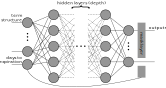
\includegraphics[width=0.9\linewidth]{architecture1}
	\caption[Network architecture with hidden layer width $K=5$]{%
		Network architecture with hidden layer width $K=5$. The mask layer just masks the first output in case there are zero days to expiration.}
	\label{fig:architecture1}
\end{figure}

\section{Evaluation}

Training a neural network to estimate a real valued vector comes down to a regression problem. This section is mainly about evaluating this chapter's approach for different configurations of hyperparameters.

\subsection{Network width, depth and normalization}

\begin{figure}
	\centering
	\begin{subfigure}{0.49\linewidth}
		\includegraphics[width=\linewidth]{approach1-ex1-loss-basic}
		\caption{}
	\end{subfigure}
	\begin{subfigure}{0.49\linewidth}
		\includegraphics[width=\linewidth]{approach1-ex1-val-basic}
		\caption{}
	\end{subfigure}
	\\
	\begin{subfigure}{0.49\linewidth}
		\includegraphics[width=\linewidth]{approach1-ex1-loss-normal}
		\caption{}
	\end{subfigure}
	\begin{subfigure}{0.49\linewidth}
		\includegraphics[width=\linewidth]{approach1-ex1-val-normal}
		\caption{}
	\end{subfigure}
	\caption[Resulting loss depending on width, depth and normalization]{The resulting loss depending on width, depth and normalization of training data. (a) Training loss without normalization; (b) Validation loss without normalization; (c) Training loss with normalization; (d) Validation loss with normalization.}
	\label{fig:approach1-ex1}
\end{figure}

\begin{figure}
	\centering
	\includegraphics[width=0.9\linewidth]{approach1-ex1-progression}
	\caption[Progression of training loss for networks with $L=1$ and $K=24$]{Progression of training loss for networks with $L=1$ and $K=24$. Mean and standard derivation (std.) over ten identical networks trained separately.}
	\label{fig:approach1-ex1-progression}
\end{figure}

For evaluating depth $L$ and width $K$ of the network as well as the influence of normalization a number of models different in these hyperparameters were trained. While the choice for normalization is a binary one, $L \in \{1,3,\dots,9\}$ and $K \in \{9,12,\dots,24\}$ were used. The training happened for 1,000 epochs\footnote{%
	One epoch specifies the number of iterations during SGD until the network as seen each sample exactly one time. For 1,000 epochs the network has seen each sample 1,000 times, subsequently.}
and for each combination ten models are trained to get information about mean and variance. A total of $2 \cdot 5 \cdot 6 \cdot 10 = 600$ models were trained.

For evaluating the results, for each model the epoch with the minimum loss was selected. Afterwards the mean over all models with identical hyperparameters was taken forming the figures in~\ref{fig:approach1-ex1}. There are three observations:

\begin{enumerate}
	\item As expected, the training loss decreases for more powerful models with larger depth and width. In contrast, the structure of the validation loss looks different. This is an example of overfitting where the network is not fitted to the problem but the training data only.
	\item Just looking at the validation loss, the performance obviously worsens with increasing depth. Only increasing the width seems to have an influence on decreasing the loss. These are similar results to \cite{Niaki-2013}.
	\item There is no obvious advantage to using normalized data. Looking at figure~\ref{fig:approach1-ex1-progression}, the network in general converges faster using normalized data but also shows higher variance. The differences are neglectable, therefore normalization is not pursued further.
\end{enumerate}


\subsection{Regularization techniques}

\begin{quote}
	``Many strategies	used in machine learning are explicitly designed to reduce the test error, possibly at the expense of increased training error. These strategies are known collectively as regularization.''\cite[p.\,228]{Goodfellow-et-al-2016}
\end{quote}

Regularization is especially important in deep learning, where it is hard to visualize and understand what exactly was learned by the network. There is a large number of regularization techniques available, some of them exclusive for neural networks. Even a simple strategy like ``stopping the training when the validation error increases'' (\emph{early stopping}) is already some kind of regularization. This section mainly focuses on comparing three approaches: The widespread \emph{dropout regularization}, \emph{self-normalizing neural networks} (using SELUs as activation functions) and an attempt on \emph{data augmentation}, using minutely data for training.\footnote{%
	Data augmentation: Creating similar -- but not identical -- data from existing one, increasing the variance and hence making the network more robust. Even though the data was not newly generated the general idea is similar. By using some minute's futures as input, targeting the spread prices of the same minute at the next term, the network would learn a similar mapping. The number of samples increases by factor 1,440.}

\begin{figure}
	\centering
	\begin{subfigure}{0.49\linewidth}
		\includegraphics[width=\linewidth]{approach1-ex3-val-minutely}
		\caption{}
	\end{subfigure}
	\begin{subfigure}{0.49\linewidth}
		\includegraphics[width=\linewidth]{approach1-ex3-val-selu}
		\caption{}
	\end{subfigure}
	\caption[Validation loss for models trained with regularization techniques]{Validation loss for models trained with (a) minutely data and (b) SELU activations.}
	\label{fig:approach1-ex3}
\end{figure}

For evaluating the effectiveness of regularization the range of width $K$ and especially depth $L$ to search over was widened, except for minutely data. Using $L \in \{1,4,\dots,91\}$ and $K \in \{3,6,\dots,33\}$ a total of $30 \cdot 30 = 900$ models were trained. The large raise of the maximum depth was done in hope of finding a network with better abstraction capabilities, since the former experiments favored shallow networks. There was only one training run per model configuration, therefore neglecting statistical soundness. 

For minutely data $L \in \{1, 4, \dots, 28\}$ and $K \in \{3,6,\dots,30\}$ were chosen. Further increasing the depth would have been computationally expensive. Because of similar reasons the batch size was set to 1024, also reducing the noise at each weight update. For each such configurations ten models were trained.

Looking at the results in figure~\ref{fig:approach1-ex3}, their implications do not seem much different from the former experiments. Again, for each model the epoch with minimum loss was selected:

\begin{enumerate}
	\item For dropout, the smallest loss was around $0.2$, much higher than all other models. Hence using dropout seems out of question. It neither allows for deeper networks nor does it result in an acceptable loss, regardless of configuration.
	\item Building self-normalizing neural networks with SELUs seems promising. But comparison with figure~\ref{fig:approach1-ex1} shows not much difference, concluding that in this case simple width is more important than some additional regularizations.
	\item Again, a small depth in connection with a large width seems to be the preferred configuration. 
\end{enumerate}

\subsection{Additional inputs}

Remembering section~\ref{sec:seasonality}, there were some additional inputs which might hold important information. Adding these inputs to the existing models might decrease the loss under the conditions that these features indeed are useful and that the model is able to learn their underlying pattern. 

Therefore two inputs are added: The corresponding day of month and the month itself, represented as simple natural numbers where January $\mapsto 1$, \dots, December $\mapsto 12$. Increasing the depth hurt performance in previous experiments, therefore depth $L = 1$ is chosen while width is set to $K \in \{20,23,\dots,50\}$. For each configuration ten models were trained, resulting in a total of $11 \cdot 10 = 110$ models. Furthermore, there were some training runs with normalized values but since the performance was always much worse these will not be evaluated further.

\begin{figure}[h!]
	\centering
	\includegraphics[width=0.9\linewidth]{approach1-ex4-val-basic}
	\caption[Validation loss using additional inputs with respect to width]{Validation loss for models with additional input. The x-axis shows the networks' width. Ten models were trained, shown by the thin lines. The thick blue line is the mean and the light blue area the standard derivation in either direction.}
	\label{fig:approach1-ex4}
\end{figure}

\newpage

The results are shown in figure~\ref{fig:approach1-ex4}. While mean and standard derivation seem reasonable, the loss itself only gains significance by comparing it to the other experiments. This is done in the following section.

\subsection{Comparison}
\label{sec:aao-comparison}

There are four models used for comparison, corresponding to the experiments described above:

\begin{enumerate}
	\item Basic network as presented in section~\ref{sec:aao-network-architecture} (Basic)
	\item Network using dropout regularization (Dropout)
	\item Self-normalizing network using SELUs (SNN)
	\item Basic network trained with minutely data (Minutely)
	\item Network with additional inputs for days and month (AddIn)
\end{enumerate}

All these networks have a depth $L=1$ and width $K=30$. Using a greater width might lead to marginally better performance. The training data is not normalized. Furthermore the learning rate is reduced by $\sqrt{0.1}$ up to two times if there is no improvement on the validation loss for 20 epochs. If there is still no improvement afterwards the training is stopped (\emph{early stopping}). As a baseline a naive prediction is used: It just assumes the futures' prices did not change for the next day, calculating spread prices and error from these.

By looking at table~\ref{tab:aao-comparison} -- especially the last column using the test dataset not used for network optimization -- the results are quite devastating. The error on most models is worse than for naive prediction. Only the self-normalizing network and the network trained with minutely data beat this by a negligible difference. Furthermore the training error is unusually high, often above the validation MSE. Even though the training data seems to have higher fluctuations -- likely because of the financial crisis in 2008 -- one could expect the networks to fit more to this dataset. Therefore this chapter's approach failed to deliver useful predictions.

\begin{table}
	\centering
	\caption[Comparison of the results obtained by the first approach]{Comparison of the results obtained by the first approach. Smaller error (MSE) indicated better performance. Because training and validation set were used for optimization the test MSE is most meaningful.}
	\begin{tabular}{llrrr}
		\toprule
		{} & Epoch &  Training MSE &  Validation MSE &  \textbf{Test MSE} \\
		\midrule
		Naive    &       &        0.2099 &          0.0985 &    0.1318 \\
		Basic    &   307 &        0.1386 &          0.1013 &    0.1563 \\
		Dropout  &   174 &        0.1895 &          0.2426 &    0.2984 \\
		SNN      &   242 &        0.1425 &          0.1077 &    \textbf{0.1259} \\
		Minutely &    70 &        0.2252 &          \textbf{0.0896} &    0.1294 \\
		AddIn    &   268 &        \textbf{0.1297} &          0.0997 &    0.1321 \\
		\bottomrule
	\end{tabular}
	\label{tab:aao-comparison}
\end{table}
\chapter[Second approach: Predicting spread prices separately]{Second approach: \\ Predicting spread prices separately}
\label{ch:one-at-once}
Since the first approach failed to deliver reasonable results, no matter the network's configuration, one may rethink the fundamentals: the data itself. The topic of this work is about the term structures formed by the futures' prices. Therefore the inputs of the network need to represent this term structure in some way and consequently are not subject to large changes. The situation is different for the output. Even though targeting spread prices seems natural, restructuring the data is certainly viable.

In this chapter the networks only have a single output. Having to predict only one value simplifies the task itself. First, the newly arranged data is described in more detail, followed by a short description of the adjusted network architecture. By evaluating and comparing the results of different experiments this chapter is concluded.

\section{Data description}

The available data is the same as in chapter~\ref{ch:all-at-once}. Therefore the properties are generally the same. The goal is to rearrange the data to simplify the learning process for the network. 

There are two obvious alternatives for ordering the spread prices to get a one-dimensional target:

\begin{enumerate}
	\item As futures are issued per month they can be be represented in this manner, forming twelve vectors corresponding the the months of a year
	\item They can also be represented in a similar manner to the first approach: as legs of a term structure, hence forming six vectors
\end{enumerate}

This chapter explores the necessary transformations and properties of these representations while also describing possible adjustments of the input data.

\subsection{Monthly representation}
\label{sec:oao-monthly-representation}

Each future has a corresponding symbol, assigning it to its month of expiration. By calculating the long spread prices using \eqref{eq:long-spread} and assigning the results the same symbol as $m_i$ one can easily filter the spreads by month. This result in a total of 15,193 values.

Looking at table~\ref{tab:spreads-by-month} there are around 1,266 values available per month with mostly similar properties. These can be used for training twelve specialized networks using the term structure as input and targeting only the corresponding month's spread price. Another advantage besides simplification is the implicit inclusion of seasonality.

\begin{table}
	\centering
	\caption[Descriptive statistics for spread prices by month]{Descriptive statistics for spread prices by month as described in section~\ref{sec:oao-monthly-representation}. Notice the outliers for November and December which can again be attributed to the 2008 financial crisis.}
\begin{tabular}{lllllllll}
	\toprule
	{} &  Count &   Mean &  Std. &    Min. &   25\% &   50\% &   75\% &  Max. \\
	\midrule
	Jan &  1281 &   0.54 &  0.67 &   -3.06 &   0.15 &   0.40 &   0.87 &  2.75 \\
	Feb &  1239 &   0.25 &  0.61 &   -1.55 &   0.00 &   0.18 &   0.35 &  4.90 \\
	Mar &  1238 &  -0.06 &  0.58 &   -3.05 &  -0.23 &  -0.05 &   0.22 &  1.55 \\
	Apr &  1329 &   0.28 &  0.53 &   -2.89 &   0.05 &   0.22 &   0.45 &  3.60 \\
	May &  1289 &   0.04 &  0.56 &   -3.97 &  -0.10 &   0.07 &   0.21 &  2.75 \\
	Jun &  1279 &   0.03 &  0.39 &   -2.24 &  -0.15 &  -0.01 &   0.16 &  1.86 \\
	Jul &  1328 &   0.32 &  0.46 &   -2.72 &   0.10 &   0.28 &   0.47 &  3.12 \\
	Aug &  1224 &  -0.13 &  0.43 &   -2.03 &  -0.30 &  -0.10 &   0.05 &  2.85 \\
	Sep &  1236 &   0.29 &  0.67 &   -7.08 &   0.09 &   0.21 &   0.45 &  3.60 \\
	Oct &  1281 &   0.31 &  0.65 &   -4.01 &   0.10 &   0.23 &   0.45 &  3.30 \\
	Nov &  1256 &   0.23 &  0.93 &  -13.68 &   0.10 &   0.24 &   0.45 &  3.54 \\
	Dec &  1213 &  -0.87 &  1.15 &  -10.90 &  -0.94 &  -0.60 &  -0.33 &  1.64 \\
	\bottomrule
	\end{tabular}
	\label{tab:spreads-by-month}
\end{table}

\subsubsection{Adjusting the input structure}

Just using the same input representation as in the first approach -- the difference over the futures prices' term structure -- leads to bad performance. The reason might be that the above mentioned seasonality can not be learned with how the data is currently structured. With futures price $m_i$ and spread price $v_i$ (of the next day) the network learns some mapping:

\begin{equation}
	\begin{bmatrix}
	m_1 & \cdots & m_8
	\end{bmatrix}^\top
	\mapsto v \in \{v_2, \dots, v_7\}
\end{equation}

On the one hand it is assured that target $v$ is the spread price of a certain month. However, there is no information about the spread's term structure included. (is it $v = v_1$ or $v = v_2$ or\dots?) On the other hand the inputs represent a term structure but do not include information about seasonality. (is $m_1$ the future of January or February or\dots?) This is solved by representing the inputs not as term structure but as a 12-dimensional vector where each index represents a month.\footnote{%
	The implementation just chooses the calendarial order where January~$\mapsto 1$, \dots, December~$\mapsto 12$.}
Since for each sample at most eight values are available, the remaining positions are handled like missing values by the network in the same way as in section~\ref{sec:aao-data-handling}. This way seasonal information is included but also the term structure by the availability of values. 

\subsection{Term structure representation}
\label{sec:oao-term-structure-representation}

An alternative representation is gained by taking the term structure of spread prices from section~\ref{sec:aao-target-data} and filtering by the individual legs. This results in six target vectors, each one with around 2,555 entries. By using these, six networks specialized on a certain leg can be trained.

\begin{table}
	\centering
	\caption[Descriptive statistics for spread prices by term structure leg]{Descriptive statistics for spread prices by term structure leg as described in section~\ref{sec:oao-term-structure-representation}.}
	\begin{tabular}{lrrrrrrrr}
		\toprule
		{} &  count &  mean &  std &    min &   25\% &  50\% &  75\% &  max \\
		\midrule
		V2 & 2790 &  0.26 & 1.27 & -13.68 & -0.13 & 0.27 & 0.79 & 3.95 \\
		V3 & 2656 &  0.18 & 0.74 &  -9.49 & -0.04 & 0.23 & 0.48 & 3.29 \\
		V4 & 2656 &  0.01 & 0.54 &  -3.25 & -0.15 & 0.09 & 0.26 & 2.10 \\
		V5 & 2629 &  0.05 & 0.50 &  -2.91 & -0.11 & 0.10 & 0.30 & 4.90 \\
		V6 & 2455 &  0.01 & 0.48 &  -3.97 & -0.15 & 0.05 & 0.20 & 2.08 \\
		V7 & 2146 &  0.13 & 0.46 &  -3.11 & -0.05 & 0.15 & 0.30 & 3.12 \\
		\bottomrule
	\end{tabular}
	\label{tab:spreads-by-leg}
\end{table}

Although no information about seasonality is included (one can not say which months or days are affected), the legs' underlying temporal information is: Spread price $v_i$ is calculated using futures prices $m_{i-1}, m_i, m_{i+1}$ \eqref{eq:long-spread}. Meaning the center of spread $v_i$ expires in around $i$ months.

Adjusting the inputs is not necessary.

\section{Network architecture}

The theory and network architecture are generally the same as in the previous chapter's section~\ref{sec:aao-network-architecture}. A mask layer is not needed since there is only a single network output for which target data is always available. Also, the same defaults for the hyperparameters are chosen, meaning ReLU activation functions, MSE for the loss, optimization with Adam and weight initializations using~\eqref{eq:glorot-initialization}.

\section{Evaluation}

For each of the two data representations described above one needs to find an optimal configuration of hyperparameters -- especially for the network's depth and width -- using the validation set. By using the found models for predictions on the test set -- possibly after some reordering -- a final evaluation can be made.

\subsection{Monthly representation's network}

By training networks with depth $L \in \{1,\dots,28\}$ and width $K \in \{3,\dots, 30\}$ for every month of the year, and an additional second training run per model to partly rule out noise, one gets a total of $10 \cdot 10 \cdot 12 \cdot 2 = 2400$ models. For evaluation, first the epoch with the minimal validation loss per model is selected. Afterwards the mean over all months is taken, allowing for generally evaluating width and depth independently of the month.

\begin{figure}
	\centering
	\begin{subfigure}{0.49\linewidth}
		\includegraphics[width=\linewidth]{approach2-diff_yearly}
		\caption{}
	\end{subfigure}
	\begin{subfigure}{0.49\linewidth}
		\includegraphics[width=\linewidth]{approach2-naive-comparison}
		\caption{}
	\end{subfigure}
	\caption[Evaluation using data in monthly representation]{Evaluation of network's performance using data in monthly representation. (a) Mean performance with respect to network width and depth. (b) Comparison of network with depth $L=1$ and width $K=30$ to naive prediction on the test set. The horizontal lines visualize the corresponding mean.}
	\label{fig:approach2-ex1}
\end{figure}

The results are shown in figure~\ref{fig:approach2-ex1}. While searching for an optimal combination of network depth and width (a) there are three findings:

\begin{enumerate}
	\item In contrast to the first approach it seams viable to increase the depth. Even with larger depth the loss seems acceptable. Furthermore there seems to be a correlation between loss and width because decreasing the width while at the same time increasing the depth stabilizes the loss.
	\item Nevertheless, the optimal combination is again depth $L=1$ and width $K=30$, albeit by a smaller margin.
	\item By comparing the predictions to a naive prediction -- assuming the spread prices are the same on the next day -- the results are disastrous. While the naive prediction is quite good with a mean of $0.04$ over all months the predictions are much worse with a mean of $0.31$. But also doing a monthwise comparison the performance of the network is always worse.
	The large difference in error between validation and test set also implies bad generalization properties.
\end{enumerate}

Even though during training the loss seemed acceptable, by validating the results on the test set the performance took a huge drop. In conclusion, the approach of using a monthly representation failed.

\subsection{Term structure representation's network}

Again, for each of the six legs of a spread prices' term structure a model with $L \in \{1,\dots,28\}$ and width $K \in \{3,\dots, 30\}$ is trained. This is repeated five times for each configuration for additional evaluation of variance. Therefore a total of $10 \cdot 10 \cdot 6 \cdot 5 = 3000$ models were trained. By first selecting the epoch with minimal validation loss per model, followed by taking the mean, one gets to evaluate depth and width as presented in figure~\ref{fig:approach2-ex2}.

\begin{figure}
	\centering
	\begin{subfigure}{0.49\linewidth}
		\includegraphics[width=\linewidth]{approach2-legwise}
		\caption{}
	\end{subfigure}
	\begin{subfigure}{0.49\linewidth}
		\includegraphics[width=\linewidth]{approach2-ex2-naive-comparison}
		\caption{}
	\end{subfigure}
	\caption[Evaluation using data represented as legs of a term structure]{Evaluation using data represented as legs of a term structure. (a) Mean performance with respect to network width and depth. (b) Comparison of network with depth $L=1$ and width $K=30$ to naive prediction on the test set. The horizontal lines visualize the corresponding mean.}
	\label{fig:approach2-ex2}
\end{figure}

The results are nearly identical to the former experiment using a monthly data representation. Most notably is the much smaller difference between the error values when comparing the networks' prediction (mean: $0.18$) and the naive prediction (mean: $0.13$). Nevertheless, beating the naive prediction did not work out, hence this approach is a failure, too.

By ordering the six networks' outputs, therefore forming a full term structure of tomorrows predicted spread prices, it is possible to make a comparison to the approach from chapter~\ref{ch:all-at-once}. Here, the resulting error is $0.176$ on the test set. Comparing this value to just the basic network from table~\ref{tab:aao-comparison} with error $0.156$ leads to the realization of the shortcomings of this approach. Dividing the work between several disconnected networks seems like a simplification, but at the end it just leads to similar or worse results. A possible cause might be the loss of context during optimization, where other outputs are not considered even if they possess a similar structure.

 


\chapter{Conclusion}
\begin{quote}
	``Most tasks that consist of mapping an	input vector to an output vector, and that are \emph{easy for a person to do rapidly}, can	be accomplished via deep learning, given sufficiently large models and sufficiently	large datasets of labeled training examples.''\cite[p.\,167]{Goodfellow-et-al-2016}
\end{quote}

Although being more of an intuition than a formal rule, above quotation might capture the reason for this work's failure. Even after simplification of the problem or after increasing the amount of training data, the network always failed to beat the simplest prediction even a human could do: To assume the next day's prices are identical to today.
Referencing section~\ref{sec:deep-learning} at the beginning of this work, even though a neural network can learn any such function, it might just learn the most obvious one.

To explore the neural network's approach to learning, one might look at an even simpler task for this work's problem: Instead predicting prices (i.e. real values) the network gets to decide a range of the next day's prices. Therefore going from a regression to a classification task.

\section{Digression: Classification approach}

The network's architecture is mostly the same as for regression. There are some differences in the choice of loss function and for some activations, but in general the network should predict if the next day's spread price is above $0.1$, below $-0.1$ or in between, resulting in three classes. The network's performance is captured by calculating its accuracy: the ratio of correctly classified samples to their total number.

Training six networks -- one for each leg of the spread prices' term structure, each with depth $1$ and width $30$ -- results in the accuracies shown in~figure~\ref{fig:classification-results}. A higher accuracy is equivalent to a better performance.
The results are quite familiar: Again, the network performs slightly worse than a native prediction (a). Even though the task is much simpler, the learned mapping is far from sophisticated. By predicting farther into the future (b) there is some interesting detail: Again the networks' performance follows the naive prediction with some gap. But at around $0.5$ accuracy the network's predictions stabilize because there seems to be a promising strategy (but surely of similar simplicity) than just approximating a naive prediction or randomly guessing. Nevertheless, this accuracy is far from satisfactory and does not justify the usage of neural networks.

\begin{figure}
	\centering
	\begin{subfigure}{0.49\linewidth}
		\includegraphics[width=\linewidth]{classification-1}
		\caption{}
	\end{subfigure}
	\begin{subfigure}{0.49\linewidth}
		\includegraphics[width=\linewidth]{classification-all}
		\caption{}
	\end{subfigure}
	\caption[Results of classification approach]{Results of classification approach using a network with depth $L=1$, width $K=1$ and three classes. The performance measure is classification accuracy, meaning higher values are better. (a) Legwise accuracy for predicting the next day. (b) Mean accuracy over all legs for predicting up to 22 days into the future.}
	\label{fig:classification-results}
\end{figure}

\section{Lookout}

The most impressive results of artificial neural networks are in areas humans are originally good at: vision, language and speech. This work was about exploring a task even humans have problems with: Financial analysis and prediction. 

Showing the shortcomings of neural networks, does this mean deep learning is useless in finance? I believe not. Finance is a vast field and because of such networks' ability to process large amounts of data and to find non-linear patterns for a possible huge number of inputs there are surely many sensible applications. Even if many of these patterns could be recognized by humans, the sheer amount of information might deem neural networks suitable. For some inspirations see \cite{DBLP:journals/corr/HeatonPW16} or \cite{Mao-2011}.
Furthermore there exist many other successful techniques -- some of classical background, some from the area of machine learning -- for different kinds of problems. A recent comparison was made in \cite{DBLP:journals/corr/QianG17}. It is choosing the right tool for the right job.

For future use of deep learning on similar problems one might consider using a much larger number of inputs. Also, \emph{self-normalizing neural networks} as shortly presented in section~\ref{sec:hyperparameters} seem to be a promising approach, provided the data satisfies the mathematical properties necessary. But most of all one needs to reconsider the end-to-end approach of deep learning like applied in other areas. Its potential in finance might be more as one part of a larger pipeline, seeing it just as one method out of many.

\printbibliography

\appendix
\chapter*{\centering Appendix}
\addcontentsline{toc}{chapter}{Appendix}
\newpage
%\setcounter{chapter}{1}
\section*{A1\hspace{1em}Example predictions by minutely network (section~\ref{sec:aao-comparison})}

\includegraphics[width=0.95\linewidth]{minutely-prediction-samples}

\section*{A2\hspace{1em}Spread prices by leg}

\includegraphics[width=0.99\linewidth]{spreads-legwise}

\section*{A3\hspace{1em}Spread prices by month}

\includegraphics[width=0.99\linewidth]{spreads-monthwise}

\section*{A4\hspace{1em}Classification network's configuration}

Hyperparameters:

\begin{itemize}
	\item Number of classes $C=3$
	\item Activation functions: Mostly ReLU (same as above). At the last layer the softmax function is used: $f(z)_j = \frac{e^{z_j}}{\sum_{i=1}^C e^{z_i}}$ where $j \in \{1,\dots,C\}$
	\item Loss function: Categorical cross entropy
	\item Optimization method: Adam (same as above)
	\item Weight initializations: Using \eqref{eq:glorot-initialization} (same as above)
	\item Network depth $L = 1$
	\item Network width $K = 30$
\end{itemize}

Furthermore, during training there is scaling applied to the loss function to reflect the imbalanced ratio of samples per category. Otherwise the network would likely learn to always predict the first category as it is overrepresented in the dataset as seen below.

\vspace{1em}

\includegraphics[width=0.9\linewidth]{classification-samples-per-category}

\end{document}          
